\documentclass[fr]{../../../../../../eplexam}
\usepackage{listings}
\definecolor{codegreen}{rgb}{0,0.6,0}
\definecolor{codegray}{rgb}{0.5,0.5,0.5}
\definecolor{codepurple}{rgb}{0.58,0,0.82}
\definecolor{backcolour}{rgb}{1.0,1.0,1.0}
\definecolor{codeblue}{rgb}{0,0,0.8}

\lstdefinestyle{mystyle}{
    backgroundcolor=\color{backcolour},   
    commentstyle=\color{codegray},
    keywordstyle=\color{codeblue},
    numberstyle=\tiny\color{codegray},
    stringstyle=\color{codeblue},
    basicstyle=\ttfamily\footnotesize,
    breakatwhitespace=false,         
    breaklines=true,                 
    captionpos=b,                    
    keepspaces=true,                 
    numbers=left,                    
    numbersep=5pt,                  
    showspaces=false,                
    showstringspaces=false,
    showtabs=false,                  
    tabsize=2,
    frame=shadowbox
}
\lstset{style=mystyle}
\lstset{language=Oz}
\hypertitle{}{4}{INFO}{1104}{2022}{Juin}{All}
{Norah Habets \and Thomas Debelle}
{P. Van Roy}

\section{kernel language}
\begin{center}
\begin{minipage}{0.45\linewidth}
Translate the following program into kernel language. Be careful to do a complete translation that uses only kernel language instructions !
\end{minipage}
%
\begin{minipage}{0.45\linewidth}
\begin{lstlisting}
local F in 
  fun {F A B}
    fun {$ C}
      fun {$ D} (A+B)*(C+D) end 
    end 
  end 
  {Browse {{{F 5 6} 4} 3}}
end
\end{lstlisting}
\end{minipage}
\end{center}

\begin{solution}
\begin{lstlisting}[escapechar=µ]
local F in
  proc {F A B R1}
  R1=proc {$ C R2}
    R2=proc {$ D R3} local V1 V2 in V1=A+B V2=C+D
      R3=V1*V2 end
      end
    end
  end
local Three Four Five Six X Y Z in Three=3 Four=4 Five=5 Six=6
  {F Five Six X} {X Four Y} {Y Three Z} {Browse Z} end
end
\end{lstlisting}
\end{solution}

\section{Give the semantic rule for the instruction "thread <s> end"}
Show the execution state before and after the execution of this instruction. Your answer can continue on the nextpage.

\begin{solution}
\begin{center}
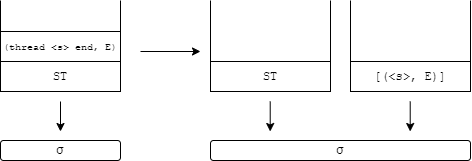
\includegraphics[scale=0.6]{Diagramme2.png}
\end{center}
Séquence d'états d'exécution: $(MST_1, \sigma_1) \rightarrow (MST_2, \sigma_2) \rightarrow ...$. MST = multiset of semantic stacks. Une étape par thread (choix du thread par le scheduler). On utilise l'interleaving semantics.\\
On crée une nouvelle pile sémantique contenant <s> et qui accède à la même mémoire que la pile sémantique de base. La mémoire est partagée.
\end{solution}

\section{Lambda calculus reduction}
Reduce the expression (SUCC (SUCC I)) and show itis equivalent to 3. Show all reduction steps. To make your answer easier to understand, you must only replace a function by its definition when you need it for a reduction step.

\begin{solution}
(SUCC (SUCC 1)) $\longrightarrow$ (SUCC ($\lambda n. \lambda f. \lambda x.f$((n f) x) 1)) $\longrightarrow$ (SUCC ($\lambda f. \lambda x.f$((1 f) x))) $\longrightarrow$ (SUCC ($\lambda f. \lambda x.f$(($\lambda f. \lambda x.fxf$)x))) $\longrightarrow$ (SUCC ($\lambda f. \lambda x.f$ (($\lambda x.fx$)x))) $\longrightarrow$ (SUCC ($\lambda f. \lambda x.f$(f x))) $\longrightarrow$ (SUCC 2) $\longrightarrow$ ($\lambda f. \lambda x.f$((2 f) x)) $\longrightarrow$ ($\lambda f. \lambda x.f(f(f$ x))) $\longrightarrow$ $3$
\end{solution}

\section{Exceptions}
To handle exceptional situations in a program, we add a new concept called exceptions. We introducenew instructions for exceptions, namely try $<s>_1$ catch $<y>$ then $<s>_2$ end and raise <x> end. For this question, give the semantics of both try and raise by showing their effects on the semantic stack. Be careful to show exactly what is on the stack, including and and also the other instructions (such as the instructions below the try). Your answer should show the connection between <x> and <y> by giving the environments of the instructions. Your answer should also show what happens in the case that no exception is raised and also what happens in the case that a raise is executed.

\begin{solution}
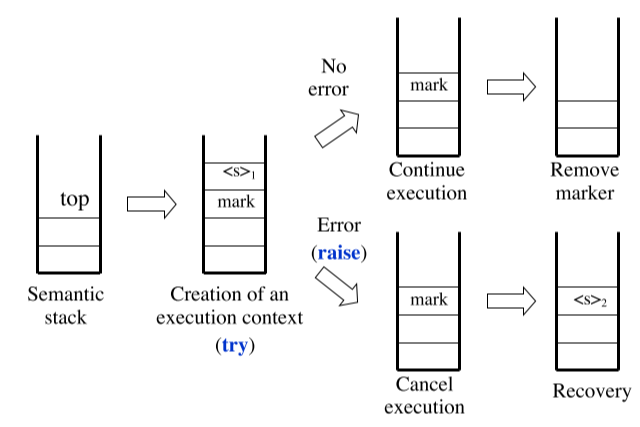
\includegraphics[scale=0.55]{stackException.png}
\end{solution}

\section{Ports and port objects}
\subsection{Give the semantics of the port send operation}
For the operation \{Send P X\}, give the execution state before and after the operation's execution. You may assume that P is correctly bound to a port before the execution (the port is already created).

\begin{solution}
En supposant que le port a été créé par P=\{NewPort S\}:
\begin{lstlisting}[escapechar=µ]
([({Send P X}, {P µ$\rightarrow$µ p, X µ$\rightarrow$µ x, S µ$\rightarrow$µ s}), ...], µ$\sigma$µ={p=µ$\xi$µ,s,x}µ$\bigcup$µ{p:s})
([(...)], µ$\sigma$µ={p=µ$\xi$µ,s=x|s',s',x}µ$\bigcup$µ{p:s'})
\end{lstlisting}
\begin{center}
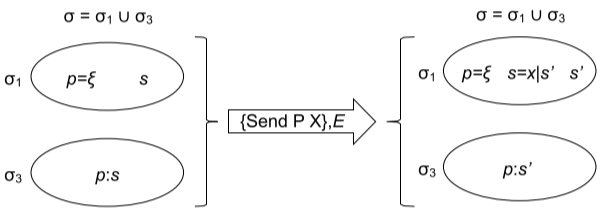
\includegraphics[scale=0.5]{semantiquePort.png}
\end{center}
\end{solution}

\subsection{Stateful port objects}
Define a function that takes an initial state and a state transition function so that it creates a stateful port Object when it is called.

\begin{solution}
\begin{lstlisting}[escapechar=µ]
fun {NewPortObject Behaviour Init}
  local S
    thread P={NewPort S} Out={FoldL S Behaviour Init} end
  in
    proc {$ M} {Send P M} end
  end
end
declare
fun {FoldL S F U}
  case S of nil then U
  [] H|T then {FoldL T F {F U H}}
  end
end
\end{lstlisting}
\end{solution}

\section{Erlang mechanisms for long-lived programs}

\subsection{Process linking}
An Erlang process is similar to a port Object. An important primitive operation to support fault tolerance in Erlang is linking, where processes are linked together. For this question, define linking and explain what it does. How does it work when there are more than processes?

\begin{solution}
Link crée un lien entre 2 processus qui est bidirectionnel dans les 2 sens. Lorsqu'un process s'arrête il envoie le signal "normal" à tous les processus auxquels il est lié, sinon il envoie la cause de son arrêt \textit{anormal}. Les processus qui reçoivent un message "anormal" crash aussi et renvoient le message causant le crash.\par 
Un process peut être configuré pour piéger les signaux de sorte en appelant \textit{process\_flag}(trap\_exit, true)\par 
Un superviseur peut recevoir dans sa mailbox le message sans s'arrêter et prendre des mesures pour restaurer le système. \par 
Ainsi, tous les processus liés au crash en suivant la chaine jusqu'à arriver au superviseur. Si aucun process ne démarre, le programme s'arrête. On peut outrepasser un superviseur avec \textbf{exit(kill, Pid)}.
\end{solution}

\subsection{Dynamic code change}
In Erlangitis possible to update the code without stopping the system. Erlang has two basic mechanisms to allow this. For this question, explain the two mechanisms and give small code fragments in Erlang to illustrate them (as we did in the course). Hint: one of the mechanisms needs to be supported by the implementation, whereas the other mechanism is a consequence of functional programming.

\begin{solution}
\begin{minipage}[t]{0.45\linewidth}
\begin{lstlisting}[language=erlang, caption={use new version}]
-module(m). 

loop(Data, F) -> 
  receive
  (From,Q} ->
    {Reply,Data1}=F(Q,Data), 
    m:loop(Data1, F)
end.
\end{lstlisting}
\end{minipage}
%
\begin{minipage}[t]{0.45\linewidth}
\begin{lstlisting}[language=erlang, caption={use old version}]
-module(m). 

loop(Data, F) -> 
  receive
  {From,Q} ->
     {Reply,Data1}=F(Q,Data), 
     loop(Data1, F)
end.
\end{lstlisting}
\end{minipage}
\end{solution}

\end{document}
